\section{Microsoft Azure Functions(刘力玮)}\label{sec:azure_use}
\subsection{基本原理}
Azure Functions是微软推出的一种无服务器计算服务,使用它可以运行事件触发的代码,而无需显式预配或管理基础结构。Azure Functions允许使用者运行小段代码(称为“函数”)且不需要担心应用程序基础结构。借助Azure Functions,云基础结构可以提供应用程序保持规模化运行所需的所有最新状态的服务器。函数由特定类型的事件“触发”。支持的触发器包括对数据更改做出响应,对消息做出响应,按计划运行,或者生成HTTP请求的结果。虽然使用者始终可以直接针对大量服务编写代码,但使用绑定可以简化与其他服务的集成。使用绑定,使用者能够以声明方式访问各种Azure服务和第三方服务。

触发器是导致函数运行的因素。触发器定义函数的调用方式,一个函数必须刚好有一个触发器。触发器具有关联的数据,这些数据通常作为函数的有效负载提供。

绑定到函数是以声明方式将另一个资源连接到该函数的一种方式;绑定可以输入绑定和输出绑定的形式进行连接。绑定中的数据作为参数提供给函数。可根据需要,混合搭配不同的绑定。绑定是可选的,一个函数可以有一个或多个输入绑定和输出绑定。图\ref{fig1}是触发器与绑定的简单实例。

\begin{figure}[!htbp]
	\centering
	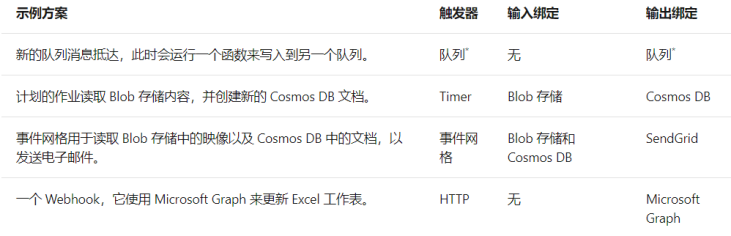
\includegraphics[scale=0.6]{figs/1.png}
	\caption{触发器与绑定实例}
	\label{fig1}	
\end{figure}

\subsection{用户手册}
下文介绍使用Visual Studio利用Azure Function开发C\#类库函数并将其发布到 Azure的技术文档。

\subsubsection{必备条件} 
从Visual Studio 2017开始,Azure Functions Tools包含在Visual Studio的Azure开发工作负荷中。确保在Visual Studio安装中包括Azure开发工作负荷并更新为最新版本,如图\ref{fig2}所示。
\begin{figure}[!htbp]	
	\centering
	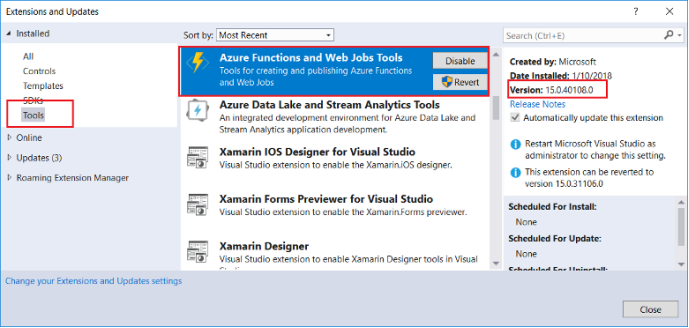
\includegraphics[scale=0.6]{figs/2.png}
	\caption{Azure开发工作负荷版本更新界面}
	\label{fig2}	
\end{figure}

\subsubsection{创建Azure Functions项目} 
Visual Studio中的Azure Functions项目模板创建一个项目,该项目可发布到Azure中的函数应用。可使用函数应用将函数分组为逻辑单元,以便更轻松地管理、部署、缩放和共享资源。
\begin{enumerate}
	\item 在Visual Studio菜单中,选择“文件” > “新建” > “项目” 。
	\item 在“创建新项目”中,在搜索框中输入“functions”,选择“Azure Functions” 模板,然后选择“下一步”。
	\item 在“配置新项目”中,输入项目的“项目名称”,然后选择“创建”。函数应用名称必须像C\#命名空间一样有效,因此请勿使用下划线、连字符或任何其他的非字母数字字符。
	\item 本例中,对于“创建新的Azure Functions应用程序”设置,使用图3中的设置,确保将“访问权限”设置为“匿名”。如果选择默认级别的函数,需要在请求中提供函数密钥才能访问函数终结点。
	\item 选择“创建”以创建函数项目和HTTP触发器函数,如图图\ref{fig3}所示。
\end{enumerate}
\begin{figure}[!htbp]
	\begin{subfigure}[b]{0.5\linewidth}
		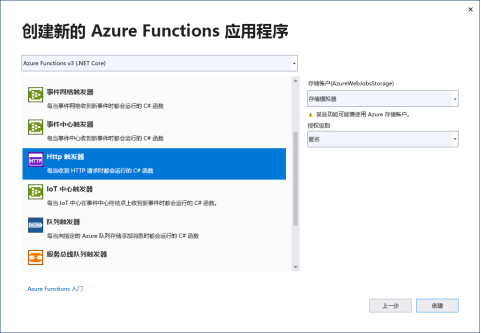
\includegraphics[width=\linewidth]{figs/3.png}
		\caption{}
		\label{fig3}
	\end{subfigure}
	\begin{subfigure}[b]{0.5\linewidth}
		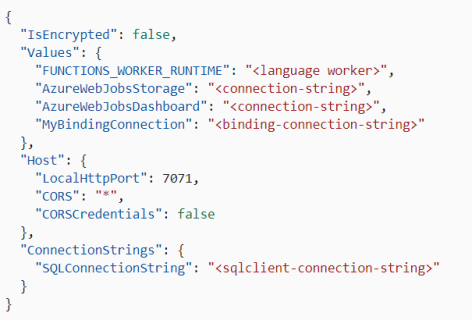
\includegraphics[width=\linewidth]{figs/4.png}
		\caption{}
		\label{fig4}
	\end{subfigure}
	\caption{(a) 创建新函数。(b) 本地设置文件结构。}
\end{figure}
此项目模板创建C\#项目,安装\texttt{Microsoft.NET.Sdk.Functions NuGet}包,并设置目标框架。新项目包含以下文件:
\begin{itemize}
	\item \texttt{host.json}:用于配置 Functions 主机。在本地和Azure中运行时,都会应用这些设置。 
	\item \texttt{local.settings.json}:维护本地运行函数时使用的设置。在Azure中运行时不使用这些设置。
\end{itemize}

\subsubsection{本地设置文件} 
local.settings.json文件存储应用设置、连接字符串和本地开发工具使用的设置。只有在本地运行项目时,才会使用 local.settings.json 文件中的设置。本地设置文件的结构如图图\ref{fig4}。

\subsubsection{将函数添加到项目} 
在C\#类库函数中,可以通过在代码中应用属性来定义函数使用的绑定。从提供的模板创建函数触发器时,将为你应用触发器属性。	
\begin{figure}[!htbp]
	\begin{subfigure}[b]{0.5\linewidth}
		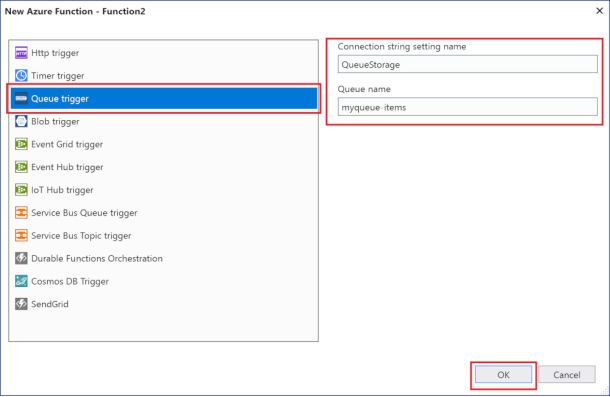
\includegraphics[width=\linewidth]{figs/5.png}
		\caption{}
		\label{fig5}
	\end{subfigure}
	\begin{subfigure}[b]{0.5\linewidth}
		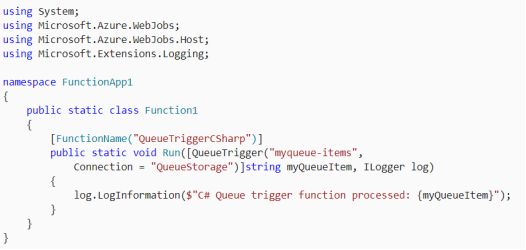
\includegraphics[width=\linewidth]{figs/6.png}
		\caption{}
		\label{fig6}
	\end{subfigure}
	\caption{(a) 添加到项目。(b) 函数代码。}
\end{figure}
\begin{enumerate}
	\item 在“解决方案资源管理器”中,右键单击项目节点,然后选择“添加” > “新建项”。选择“Azure函数”,输入类的名称,然后单击“添加”,如图图\ref{fig5}所示。
	\item 选择触发器,设置绑定属性,然后单击“创建”。以下示例显示创建队列存储触发的函数时的设置。此触发器示例使用具有名为QueueStorage的键的连接字符串。必须在web.config文件中定义此连接字符串设置。
	\item 检查新添加的类。将会看到一个静态Run方法,它已使用FunctionName属性设置了属性。该属性指示该方法是函数的入口点。图\ref{fig6}中的C\#类表示一个基本的队列存储触发的函数。	
\end{enumerate}
已向提供给入口点方法的每个绑定参数提供了特定于绑定的属性。该属性采用绑定信息作为参数。在上面的示例中,第一个参数应用QueueTrigger属性,表示队列触发的函数。 队列名称和连接字符串设置名称作为参数传递到“QueueTrigger”属性。

\subsubsection{添加绑定} 
使用触发器时,输入和输出绑定是作为绑定属性添加到函数的。
\begin{enumerate}
	\item 确保已为本地开发配置项目。
	\item 为特定绑定添加适当的NuGet扩展包。有关详细信息,请参阅“触发器和绑定”一文中的使用Visual Studio进行本地C\#开发。 特定于绑定的NuGet包要求位于绑定的参考文章中。 例如,可以在事件中心绑定参考文章中找到事件中心触发器的包要求。
	\item 如果有绑定需要的应用设置,请将其添加到本地设置文件中的Values集合。当函数在本地运行时,会使用这些值。当函数在Azure的函数应用中运行时,会使用函数应用设置。
	\item 将适当的绑定属性添加到方法签名。在图\ref{fig7}的示例中,一条队列消息触发了该函数,而输出绑定则创建了一条新的队列消息,在不同的队列中使用了相同的文本。
\end{enumerate}	
\begin{figure}[!htbp]
	\centering
	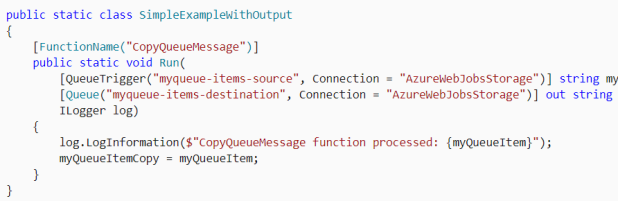
\includegraphics[scale=0.6]{figs/7.png}
	\caption{绑定实例}
	\label{fig7}	
\end{figure}

\subsubsection{函数测试} 
\begin{enumerate}
	\item Azure Functions Core Tools允许在本地开发计算机上运行Azure Functions项目。
	\item 在运行项目时,可以像测试已部署的函数一样测试代码。
\end{enumerate}	

\subsubsection{发布到Azure} 
从 Visual Studio 发布时,使用以下两种部署方法之一。Web部署:将Windows应用打包并部署到任何IIS服务器。启用了从包运行的Zip部署:建议用于Azure Functions部署。
\begin{figure}[!htbp]
	\begin{subfigure}[b]{0.5\linewidth}
		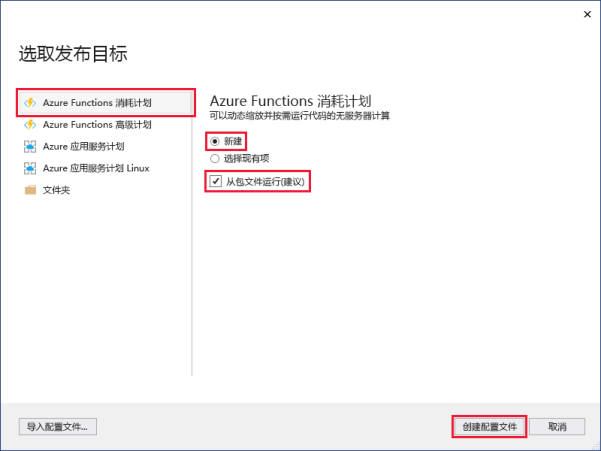
\includegraphics[width=\linewidth]{figs/8.png}
		\caption{}
		\label{fig8}
	\end{subfigure}
	\begin{subfigure}[b]{0.5\linewidth}
		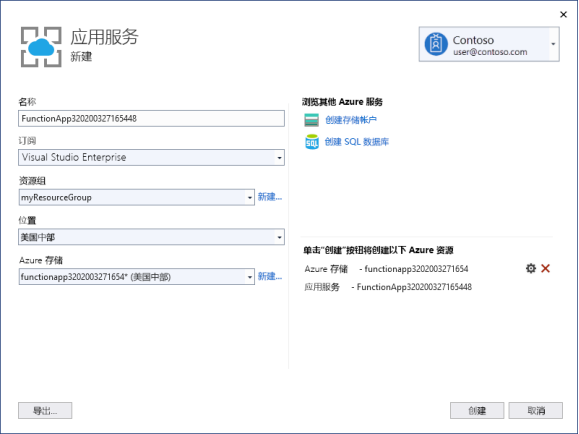
\includegraphics[width=\linewidth]{figs/9.png}
		\caption{}
		\label{fig9}
	\end{subfigure}
	\begin{subfigure}[b]{\linewidth}
		\centering
		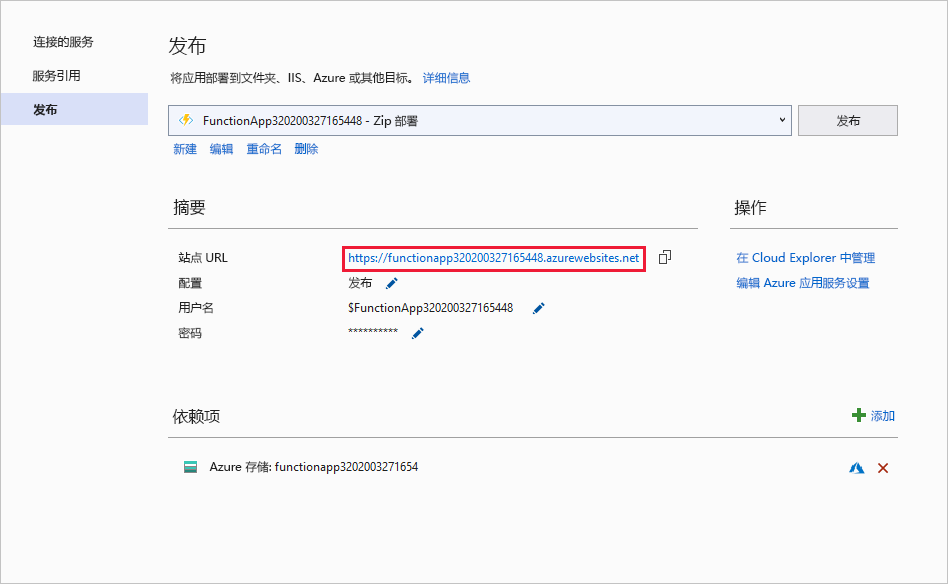
\includegraphics[width=0.6\linewidth]{figs/10.png}
		\caption{}
		\label{fig10}
	\end{subfigure}
	\caption{(a) 发布界面。(b) 应用服务界面。}
\end{figure}
本例中使用以下步骤将项目发布到 Azure 中的函数应用。
\begin{enumerate}
	\item 在“解决方案资源管理器” 中,右键单击该项目并选择“发布” 。
	\item 在“选取发布目标” 中,使用图\ref{fig8}中指定的发布选项。
	\item 选择“创建配置文件”。如果尚未从Visual Studio登录到Azure帐户,选择“登录”。也可以创建免费Azure帐户。
	\item 在“应用服务: 新建”中,使用图\ref{fig9}中指定的值。
	\item 选择“创建” ,使用这些设置在Azure中创建函数应用及其相关的资源,并部署函数项目代码。
	\item 选择“发布”,并且在完成部署后记下“站点URL” 值,这是函数应用在Azure中的地址,如图图\ref{fig10}所示。
\end{enumerate}


\subsubsection{函数应用设置} 
必须将在local.settings.json中添加的任何设置添加到Azure函数应用中。 发布项目时,不会自动上传这些设置。

将所需设置上传到Azure中的函数应用的最简单方法是使用“管理应用程序设置...”链接,如图\ref{fig11}所示。

这会显示用于函数应用的“应用程序设置”对话框,可以在其中添加新应用程序设置或修改现有设置,如图\ref{fig12}所示。
\begin{figure}[!htbp]
	\begin{subfigure}[b]{0.5\linewidth}
		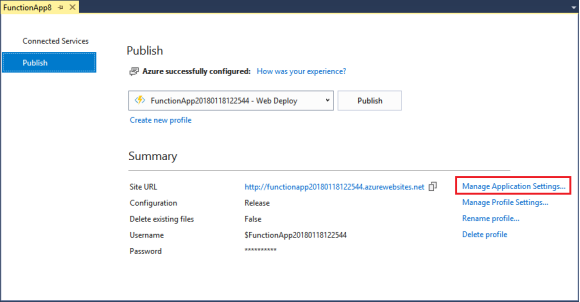
\includegraphics[width=\linewidth]{figs/11.png}
		\caption{}
		\label{fig11}
	\end{subfigure}
	\begin{subfigure}[b]{0.5\linewidth}
		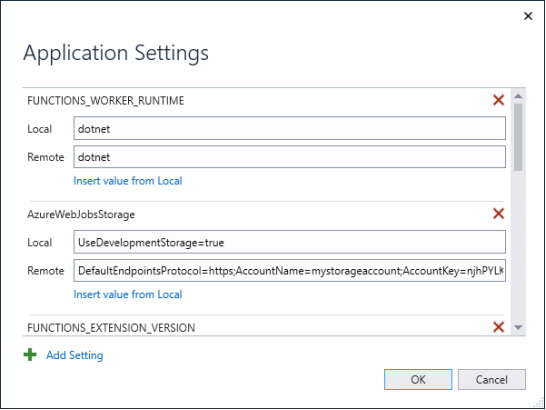
\includegraphics[width=\linewidth]{figs/12.png}
		\caption{}
		\label{fig12}
	\end{subfigure}
	\caption{(a) 函数设置界面。(b) 应用设置。}
\end{figure}

本地表示local.settings.json文件中的设置值,远程是Azure的函数应用中的当前设置。 选择"添加设置"以创建新的应用设置。使用“从本地插入值”链接将设置值复制到“远程”字段。 你选择“确定”后,挂起的更改将写入本地设置文件和函数应用。

\subsubsection{函数监视} 
监视函数执行的建议方法是将函数应用与Azure Application Insights集成。Azure Application Insights可以收集日志、性能和错误数据,自动检测性能异常,并提供强大的分析工具来帮助你诊断问题并了解函数的使用方式。

在Azure门户中创建函数应用时,默认情况下会为你完成此集成。 但在Visual Studio发布期间创建函数应用时,Azure中的函数应用集成未完成。可以通过 Functions 轻松地将Application Insights集成从 Azure门户添加到某个函数应用。
\begin{enumerate}
	\item 在Azure门户中,搜索并选择"function app",然后选择函数应用。
	\item 选择窗口顶部的 "未配置 Application Insights标题"。如果看不到此横幅,则你的应用已启用Application Insights。
	\item 使用图\ref{fig13}中的表中指定的设置创建Application Insights资源。
	\begin{figure}[!htbp]
		\centering
		
\includegraphics[scale=0.6]{figs/13.png}
		\caption{资源设置}
		\label{fig13}	
	\end{figure}
	\item 选择“应用”。Application Insights资源在与函数应用相同的资源组和订阅中创建。
\end{enumerate}	

\section{Google Cloud Functions(刘力玮)}\label{sec:google_use}
\subsection{基本原理}
Google Cloud Functions是用于构建和连接云端服务的一种无服务器执行环境。借助Cloud Functions,使用者可以编写单一用途的简单函数,并将这些函数关联到云端基础架构和服务发出的事件。当所监控的事件发生时,就会触发使用者的函数。使用者的代码将在完全托管的环境中执行。使用者无需预配任何基础架构,也不必费心管理任何服务器。

\subsection{用户手册}	
下文介绍了如何使用Cloud Console创建和部署用Python编写的Cloud Functions函数。当此函数通过HTTP请求触发时,会如图\ref{fig14}所示输出一条消息:

\begin{figure}[!htbp]
	\centering
	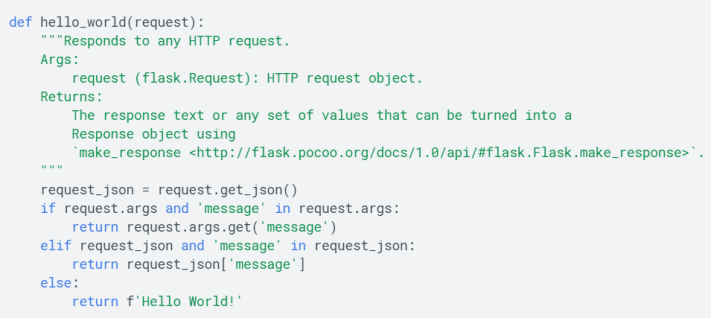
\includegraphics[width=0.7\linewidth]{figs/14.png}
	\caption{函数代码}
	\label{fig14}	
\end{figure}	

\begin{multicols}{2}
	\subsubsection{准备工作} 
	\begin{enumerate}
		\item 在Cloud Console的项目选择器页面上,选择或创建Cloud项目。
		\item 确保Google Cloud项目已启用结算功能。
		\item 启用Cloud Functions API。
	\end{enumerate}
	
	\subsubsection{创建函数} 
	\begin{enumerate}
		\item 在Cloud Console中打开Cloud Functions概览页面,如图\ref{fig15}所示。
		\item 选择启用了Cloud Functions的项目。
		\item 点击创建函数。
		\item 指定函数名称。
		\item 在触发器字段中,选择HTTP。
		\item 在源代码字段中,选择内嵌编辑器。
		\item 用运行时下拉列表选择 Python 运行时。
	\end{enumerate}
	\begin{figure}[H]
		\centering
		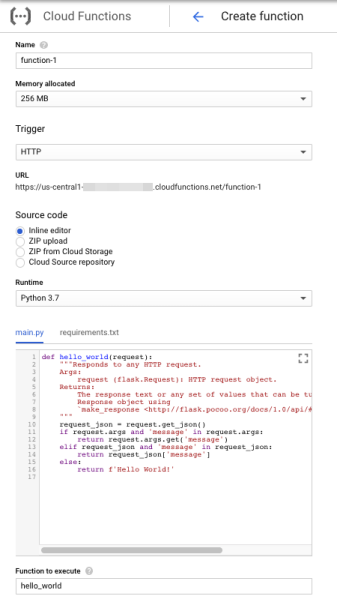
\includegraphics[width=\linewidth]{figs/15.png}
		\caption{创建函数界面}
		\label{fig15}	
	\end{figure}
\end{multicols}

\subsubsection{函数部署} 
部署的运行方式是将包含函数源代码的归档上传到Google Cloud Storage存储分区。使用者可以从本地机器、GitHub或Bitbucket源代码库(通过Cloud Source Repositories)或直接从Cloud Functions API部署Cloud Functions函数。

本例中按照以下方式:
\begin{enumerate}
	\item 点击图\ref{fig16}页面底部的创建。
	\begin{figure}[!htbp]
		\centering
		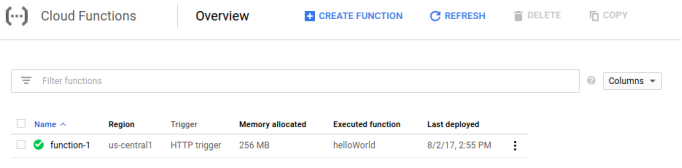
\includegraphics[scale=0.6]{figs/16.png}
		\caption{函数部署界面}
		\label{fig16}	
	\end{figure}
	\item 点击创建后,Cloud Console将重定向到Cloud Functions概览页面。
\end{enumerate}	

\subsubsection{函数测试} 
\begin{enumerate}
	\item 显示使用者的函数对应的菜单,然后点击图\ref{fig17}测试函数。
	\begin{figure}[!htbp]
		\centering
		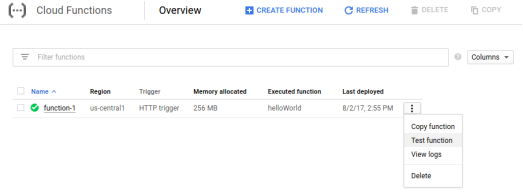
\includegraphics[scale=0.6]{figs/17.png}
		\caption{函数测试界面}
		\label{fig17}	
	\end{figure}
	\item 在测试页面上,点击测试函数。输出屏幕会显示文本 "Hello World!"
	\item 现在更改此消息。在触发事件字段中,输入文本 {"message":"Hello, YOURNAME!"}(将 YOURNAME替换为一个名字),然后点击测试函数。
	
	例如,假设输入的名字是“Rowan”。在输出字段中,会看到消息 Hello, Rowan!。在日志字段中,如果状态码为 200,则表示函数已成功执行,如图\ref{fig18}所示。
	\begin{figure}[!htbp]
		\centering
		
\includegraphics[scale=0.6]{figs/18.png}
		\caption{函数测试日志}
		\label{fig18}	
	\end{figure}
\end{enumerate}	

\subsubsection{日志查看} 
Google Stackdriver提供了一套监控工具。Stackdriver Logging可捕获并存储Cloud Functions函数日志,会捕获特殊格式的错误日志,并将其显示在Error Reporting信息中心中。

检查日志以通过日志历史记录了解函数的操作,如图\ref{fig19}所示。
返回Cloud Functions“概览”页面,显示使用者的函数对应的菜单,然后点击查看日志。
此时将显示函数的日志历史记录。
\begin{figure}[!htbp]
	\centering
	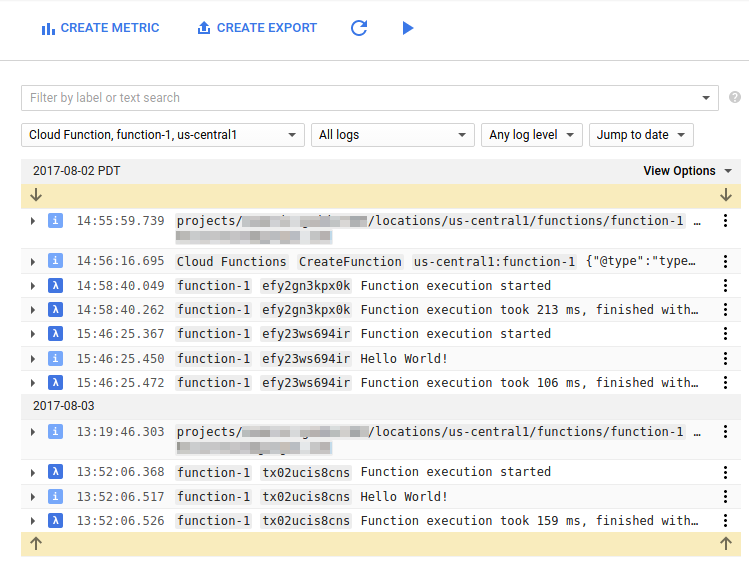
\includegraphics[scale=0.6]{figs/19.png}
	\caption{日志查看}
	\label{fig19}	
\end{figure}
